% Chapter Template

\chapter{Pile Up Studies} % Main chapter title

\label{Chapter 6} % Change X to a consecutive number; for referencing this chapter elsewhere, use \ref{ChapterX}

\lhead{Chapter 6 \emph{PU Studies}} % Change X to a consecutive number; this is for the header on each page - perhaps a shortened title

%----------------------------------------------------------------------------------------
%	SECTION 1
%----------------------------------------------------------------------------------------

\section{Jet}
\subsection{Efficiencies}
In order to test the jet finding algorithm the first study that must be undertaken is into the matching efficiency of the L1 jets to generator level quantities (gen jets). A simulated sample of $t\bar{t}$ pairs was used\footnote{In the report all simulated samples usedh ave conditions of $13TeV$ collisions with bunch spacing $50ns$. The pileup is taken to be gaussian distributed around $40$ interactions per bunch crossing}. The gen jets are made by running the anti-kt4 algorithm on the generator level quantities. The gen jet is said to be matched if it is within ${\Delta R}^2<33$ of a L1 jet (the greatest extent of the L1 jet). The matching efficiency for alljets and the fourth jet is shown in figure \ref{match}. It can be seen that the efficiency after PUS/seed drops at low $p_T$ this motivates a cut at $30GeV$ for calculation of energy sums. Inefficiencies at high $p_T$ are caused by the 'chain veto', however, the jet algorithm guarantees there is always a comparable or higher jet in the event in such cases. The performance compared to GCT is seen to be greatly improved.  
\begin{figure}
\hfill
\subfigure[All jets\label{fig:label:alljet}]{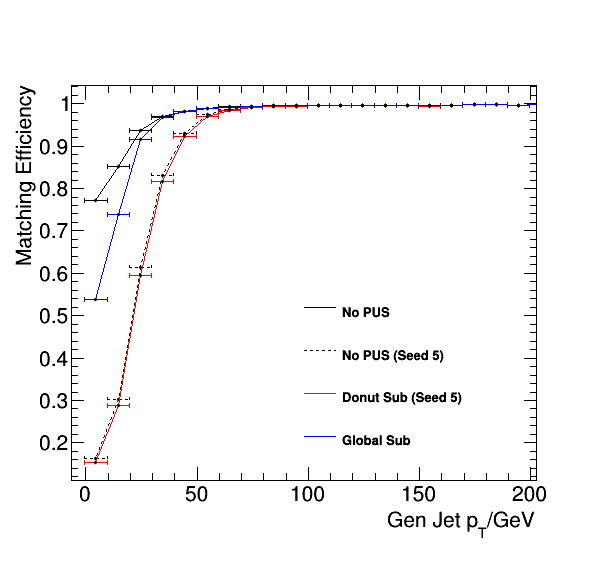
\includegraphics[width=7cm]{Figures/alljet}}
\hfill
\subfigure[4th jet\label{fig:label:jet4}]{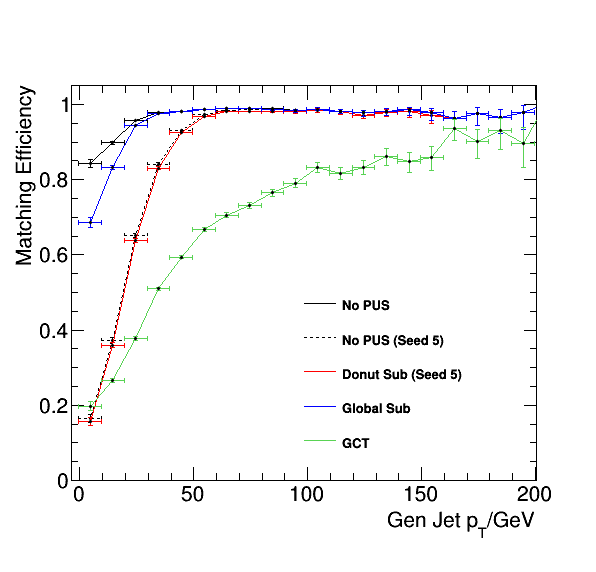
\includegraphics[width=7cm]{Figures/jet4}}
\hfill
\caption{Matching efficiencies for jets showing effect of seed and PUS at low energies. In \ref{fig:label:jet4} a comparison with the GCT is shown.}
\label{match}
\end{figure}
\subsection{Calibration}
The energy of the L1 jets is calibrated using generator level quantities. The scheme for calibration is outlined in \cite{l1jet_calibration}. The calibration is carried out in bins of $\eta$ to account for the difference in performance of the detector. Essentially, using a QCD sample, the response (defined as $p^{L1}_{T}/p^{gen}_{T}$) and $p^{L1}_{T}$ are plotted against $p^{gen}_{T}$ and fitted. The fits are then plotted against each other and the result itself fitted giving calibration factors as a function of $p^{L1}_{T}$.  Where the matching efficiency is low it is not possible to fit and so the calibration has a lower bound on $p_T$. This was found to occur at $30GeV$. An upper bound is defined by where the fits become statistically limited. This was found to occur at $300Gev$. If the fit is well defined the calibration factor should flatten with increasing $p_T$ and so higher $p_T$ jets may still be calibrated by continuing the fit. The calibration factors change depending on the PUS regime. In figure \ref{calib} the effect of the calibration is shown.   

\begin{figure}
\centering
    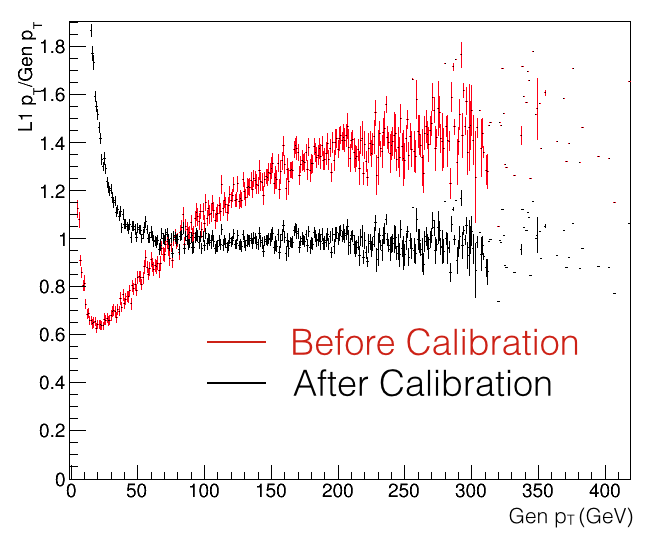
\includegraphics[width=0.9\textwidth]{./Figures/calibration}
  \caption{Effect of calibration on donut subtracted jets. At the limit of calibration ($30GeV$) the difference for the calibrated sample is around $10\%$.}
  \label{calib}
\end{figure}
\section{PUS Testing}

\subsection{Resolution dependence on number of interactions}

In this section plots are shown for the highest $|\eta|$ bin as the detector performance is expected to worsen with larger $|\eta|$ and so PUS will have the largest effect. The first test of any PUS scheme is the effect on the resolution. In an ideal post PUS scenario this will be flat as a function of the number of interactions. In figure \ref{fig:label:resolution1} this is plotted for a particular $p^{gen}_T$ and $\eta$ bin. It can be seen that the response flattens for both PUS regimes. This is summarised in \ref{fig:label:resolution2} where the gradient from the fit to the resolution plot is shown to reduce after PUS for a range of $p^{gen}_T bins$.  
\begin{figure}
\hfill
\subfigure[\label{fig:label:resolution1}]{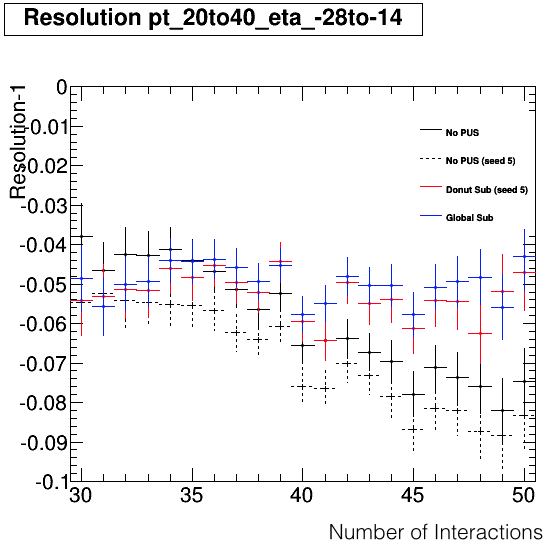
\includegraphics[width=7cm]{Figures/resolution}}
\hfill
\subfigure[\label{fig:label:resolution2}]{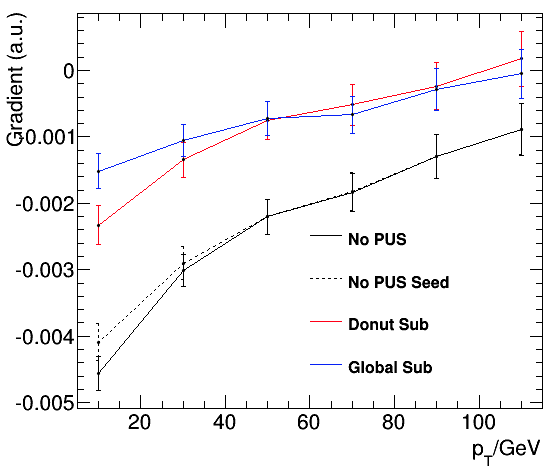
\includegraphics[width=7cm]{Figures/p1eta_14to28_calib_fits}}
\caption{In \ref{fig:label:resolution1} response versus number of interactions is shown for a particular eta bin showing the response flattens after PUS. In \ref{fig:label:resolution2} the fit gradient for different $p_{T}$ bins is shown.}
\label{fig:label:resolution}
\end{figure}
\subsection{Rates}
The rate is defined as the proportion of jets for background passing a particular $p_{T}$ cut. For the efficiency a cut is made on the gen jets ($50GeV$). The proportion of these events with a corresponding matched L1 jet over a threshold then defines the efficiency at that threshold.  For the trigger the key test is to see that the efficiency for signal may be maintained while reducing the background rate. For the background a pure pileup sample was used while the $t\bar{t}$ samples was used for signal. In figure \ref{fig:label:ratejet1} the rate is shown for the leading jet. The performance compared to the GCT is shown to be improved. The seed cut appears to have the largest effect in reducing the rate as global is shown to be comparable to no PUS. Figure \ref{fig:label:ratenvtx} shows the evolution of the rate with the number of interactions. GCT shows the largest dependence, as expected, while for stage 2 PUS is shown to flatten this dependence. Applying donut subtraction appears to increase the rate compared to applying a seed alone. This may be due to contamination causing over subtraction. The calibration will then bring the energy above the seed. Finally, in figure \ref{fig:label:rateeff} the seed is shown to be comparable to global alone while applying donut subtraction worsens the performance. This may be due to over-subtraction of jets due to contamination for nearby jets in the donut ring.
\begin{figure}
\hfill
\subfigure[Rate Jet 1\label{fig:label:ratejet1}]{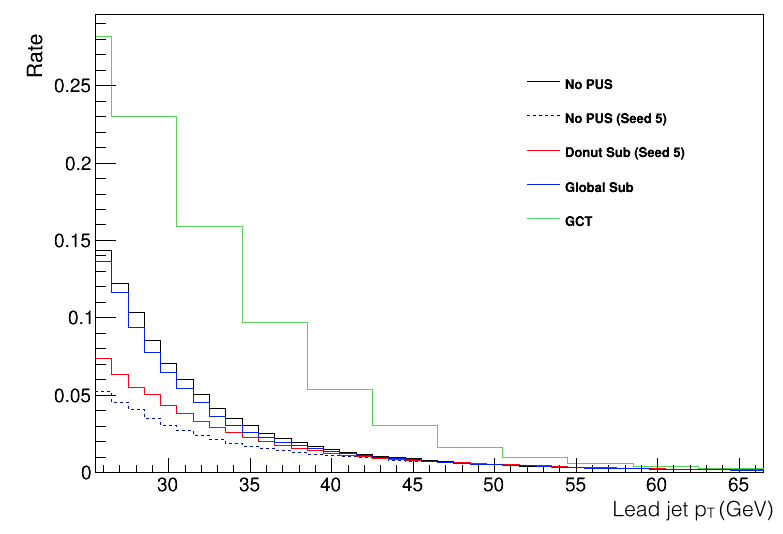
\includegraphics[width=7cm]{Figures/rate_jet1}}
\hfill
\subfigure[Rate Jet 1\label{fig:label:ratenvtx}]{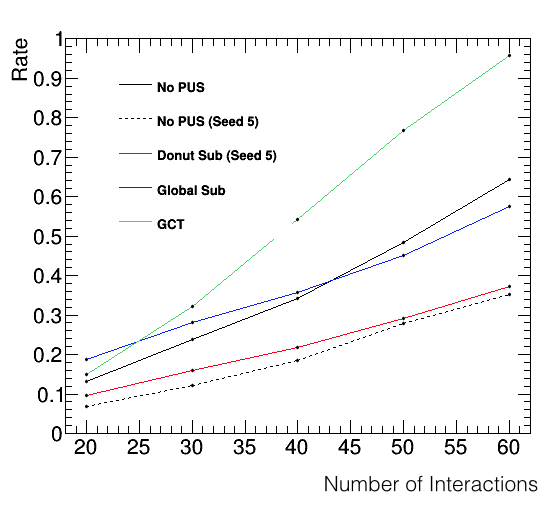
\includegraphics[width=7cm]{Figures/neutrinonvtx_jet1}}
\caption{The dependence of the rates for the lead jet with $p_T > 30 GeV$ on the number of interactions is shown in figure \ref{fig:label:ratenvtx} while\ref{fig:label:ratejet1} shows improved rate for stage 2 compared to GCT and for PUS.}
\label{fig:label:rates}
\end{figure}
\begin{figure}
\centering
    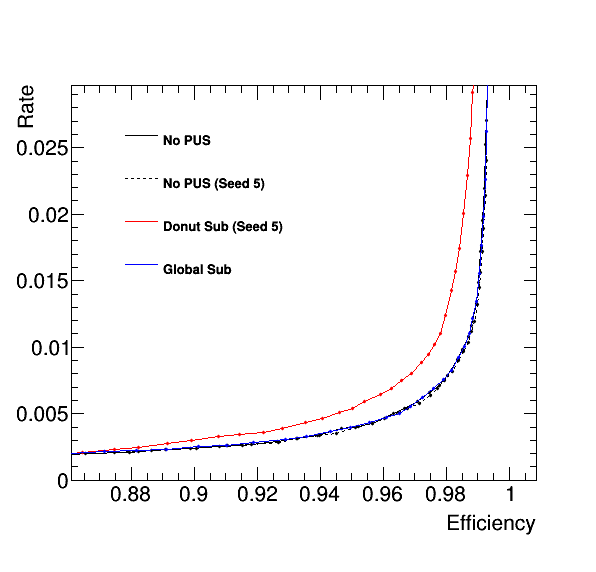
\includegraphics[width=10cm]{./Figures/jet1RateEff}
  \caption{Rate versus efficiency for lead jet. Performance is consistent except for donut which appears to excessively reduce efficiency}
  \label{fig:label:rateeff}
\end{figure}
\subsection{Turn On Plots}
To benchmark the performance of the L1 jets their $p_T$ must be compared with matched generator level quantities. To do this the generator level quantity is plotted with a cut on the matched L1 quantity (the turn on). This is shown for two representative examples in figure \ref{turnon}. As can be seen the turn on for the GCT is less sharp than that for the stage 2 quantities. Donut subtraction is seen to be inefficient at higher $p_T$ values. This suggests contamination for nearby jets or fluctuations in the donut ring causes such jets to have lower $p_T$.
\begin{figure}
\centering
    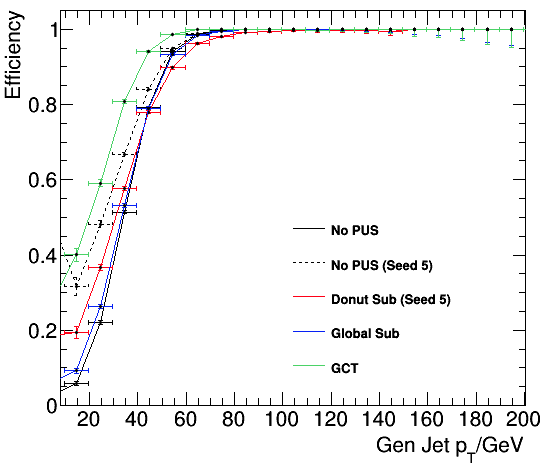
\includegraphics[width=0.8\textwidth]{Figures/jet4_40}
  \caption{Turn on curve for the 4th jet at 40 GeV showing comparable behaviour for the stage 2 quantities and a shallower turn on for GCT.}
  \label{turnon}
\end{figure}
\subsection{Energy Sums}
Lastly the energy sums which are used to make triggers based $H_T$ and $\cancel{H_T}$ were investigated. To nullify the problem of the lower calibration limit, only jets above this are included in the sums. Pileup is expected to be approximately uniform and so it should not affect the missing energy in the event. The result for $H_T$ and $\cancel{H_T}$ for a ttbar sample are shown in figure \ref{fig:label:sums}. PUS improves the agreement as compared to gen.  The $H_T$ shows especially good agreement with gen for the case of a seed as compared to global. This is due to the under-subtraction bias of the global rho method. The $\cancel{H_T}$ shows similar levels of agreement for all cases as expected. 
\begin{figure}
\hfill
\subfigure[$H_T$\label{fig:label:ht}]{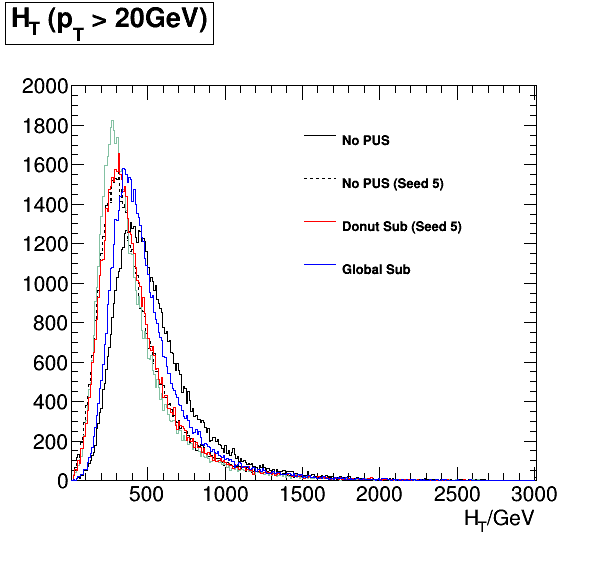
\includegraphics[width=7cm]{Figures/ht_ttbar}}
\hfill
\subfigure[$\cancel{H_T}$\label{fig:label:mht}]{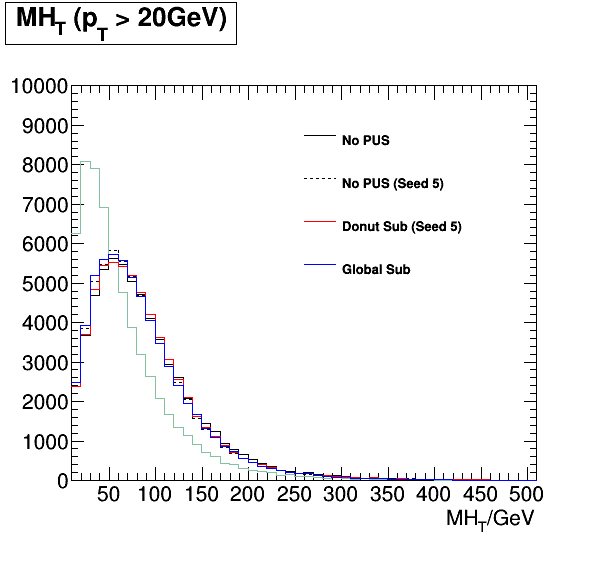
\includegraphics[width=7cm]{Figures/mht_ttbar}}
\caption{In figure \ref{fig:label:ht} the total energy shows good agreement with the generator level quantity. This is improved by requiring a seed threshold. In figure \ref{fig:label:mht} similar agreement is shown for all cases}
\label{fig:label:sums}
\end{figure}
\section{Conclusions}
The jet algorithm has been shown to function well, giving very compatible results with the offline anti-kT algorithm and maintaining a high matching efficiency to generator level quantities. The PUS studies have shown that PUS is required for run 2. While both global and donut subtraction have been shown to flatten the response (\ref{fig:label:resolution} each has weaknesses that must be addressed. Figure \ref{fig:label:rateeff} shows that applying a seed threshold is comparable to global subtraction at killing rate while maintaining efficiency. Donut subtraction is shown to perform less well than applying the seed threshold alone. This is due to the susceptibility of donut subtraction to fluctuations and contamination. Further studies are underway to increase the sampling area for donut subtraction to reduce this issue. Figure \ref{fig:label:sums} shows global $\rho$ under-performing for the $H_T$. This is due to the under-subtraction bias leading to more energy being left in the event. This may be correcting by applying a seed threshold as for donut but calculating $\rho$ using all jets. 

Further studies are currently underway to utilise the $\eta$ dependence of the pileup.  The seed threshold applied may be altered depending on the location of the tower to further reduce rate in areas of high pileup while maintaining efficiency in low pileup regions. Improving calibrations such that lower energy jets may be utilised ( the current limit is 20GeV) is also key. Finally, increasing the sample size to use $3\times3$ towers for the seed should improve discrimination between pileup and boosted jets. 

    
